\documentclass[a4paper,12pt]{article}
\usepackage{wisebed-tr}
\usepackage{placeins}
\usepackage{longtable}
\urlstyle{same}



\newenvironment{apidoc}[6]%
{%

		\begin{longtable}[t]{p{2cm}p{12.8cm}}
      Semantics	 & #2 \\[0.5em]
	    Signature	 & \lstinline{#1}\\[0.5em]
	    Parameters & {#3} \\[0.5em]
      Returns		 & #4 \\[0.5em]
      Rationale \tabularnewline for changes & #5 \\[0.5em]
      Since 		 & #6 \\[0.5em]
		\end{longtable}

 	
%	}
	\begingroup
%  }%
%  {
  \endgroup
}	


\newcommand{\apiparameters}[1]	{\hspace{-0.25cm}\begin{tabular}[t]{lp{10cm}} #1 \end{tabular}}

\newcommand{\apiparam}[2]	{ \lstinline{#1} & #2 \\ }

	
	\delivNumber{TR-SNAA-API-V1}
	\delivTitle{Sensor Network Authentication and Authorization API (SNAA API)}
	\delivAuthor{UZL, UBERN, ULANC, CTI}
	\delivDate{\today}

%---------------------------------------------------------
%  	Document Start 
%---------------------------------------------------------

\begin{document}
    \prepareTitle

%---------------------------------------------------------------------------
	\section{Introduction}
	\label{sec:introduction}
%---------------------------------------------------------------------------
This document describes the Sensor Network Authentication and Authorization API (SNAA API). This API is part of a larger family of APIs which are defined by the WISEBED consortium for reserving, accessing, managing, and using a testbed. The SNAA API is responsible for authentication of and their authorization for reserving, accessing, and using (parts of) a (potentially federated) testbed. All APIs are specified as standard Web Services using WSDL documents and a human-readable documentation. The Web Services comply to the WS-Interoperability Basic Profile~\cite{wsi-basic-profile-1-1}. All these APIs are ``federatable'' (cf. Section~\ref{sec:federatability}). At present, the following APIs exist:

\begin{itemize}
	\item Sensor Network Authentication and Authorization (SNAA API)
	\item Reservation System (RS API)
	\item Wireless Sensor Network API (WSN API) including its Sub-APIs:
	\begin{itemize}
		\item Session Management API
		\item Controller API
	\end{itemize}
\end{itemize}

Concerning implementations of this API, WISEBED already provides a set to choose from. The SNAA is implemented for authentication and authorization against a Shibboleth~\cite{shibboleth} federation, the Java Authentication and Authorization System, plain text password files, and a ''null`` implementation which grants full access for anybody. For further information and download links, please refer to \url{http://www.wisebed.eu}.

The remainder of this document is structured as follows. The remainder of this document is structured as follows. Section~\ref{sec:concepts} introduces standard concepts used throughout WISEBED, Section~\ref{sec:operations} describes the individual Web Service Operations, and Section~\ref{sec:appendix} contains the WSDL description and XML Schema document containing the data types.

%---------------------------------------------------------------------------
	\section{Concepts}
	\label{sec:concepts}
%---------------------------------------------------------------------------

%---------------------------------------------------------------------------
	\subsection{Node addressing}
	\label{sec:addressing}
%---------------------------------------------------------------------------
WISEBED uses Uniform Resource Names (URNs) to identify sensor nodes, node capabilities, edge attributes, node attributes, testbed portal servers, and 
points of interest. For more details, we refer the reader to WISEBED Deliverable D2.2 (Report on the Implementation of the Software Infrastructure) on \url{http://www.wisebed.eu}.

We define \textit{sensor nodes }as the unique nodes comprising each of the testbeds. Each sensor node belongs to only one \textit{sensor network}. A partner \textit{site} can be comprised of a number of such sensor networks. So, each sensor node of the federation is described using the unique ID of the partner site, a sensor network ID which is unique in the partner site namespace, and the sensor node ID which is unique in the specific sensor network scope it belongs to. 

\begin{lstlisting}
<URN> ::= ``urn:wisebed:node:<site>:<node id>''
\end{lstlisting}\medskip

\noindent Example: 

\begin{lstlisting}
urn:wisebed:node:cti:gw1:n1
urn:wisebed:node:cti:gw1:n8
urn:wisebed:node:uzl:building64:n33
urn:wisebed:node:ulanc:n876
\end{lstlisting}\medskip

A number of nodes share a common \emph{URN prefix}, e.g. urn:wisebed:node:cti or urn:wisebed:node:ulanc.

%---------------------------------------------------------------------------
	\subsection{Federatability}
	\label{sec:federatability}
%---------------------------------------------------------------------------
From a user's perspective, it must not matter whether he uses a local, small-scale testbed or a worldwide federation of testbeds -- or even a simulated testbed. This requires an architecture where a single testbed has the same interface towards the user as a federation of testbeds. It is therefore imperative that all interfaces, data formats, and interaction patterns are exactly the same -- independent of the type of the testbed. The goal is to come up with a generalized architecture that, amongst others, can be used 

\begin{itemize}
	\item to integrate additional testbeds in the federation, 
	\item to run private testbeds using the same APIs and their implementations,
	\item that allows third parties to operate their own testbeds (from desktop-size to a full-blown experimental facility), and 
	\item that supports the integration of simulated nodes into the experiment. 
\end{itemize}

An important aspect is that the APIs (and therefore also their implementations) are ``federatable''. Figure~\ref{fig:federation} further illustrates this concept. Here, a number of testbeds comprised of heterogeneous wireless sensor nodes are shown (a simplified WISEBED federation, a third-party testbed, and a simulated testbed using Shawn). 

 \begin{figure*}[htb]
      \begin{center}
      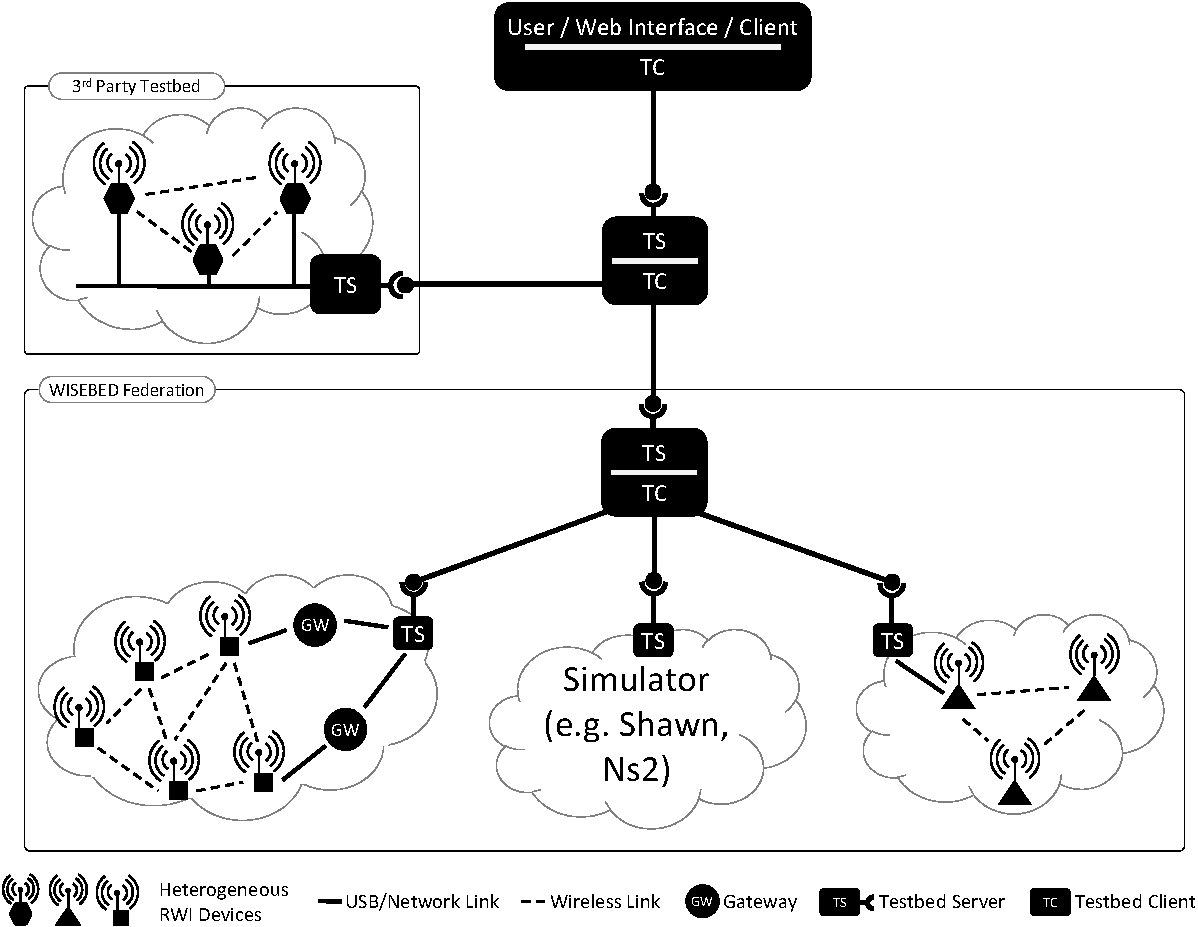
\includegraphics[width=.9\textwidth]{fig/federation}
      \caption{Federation hierarchy}
      \label{fig:federation}
      \end{center}
\end{figure*}

Each testbed (with or without a wired backbone or simulated) exposes its features using Web Services to the Internet (labeled Testbed Server, TS). Each client (Testbed Client, TC) uses these APIs to access the testbed (including AAA, reservation, reprogramming of nodes, sending messages to/receiving messages from nodes, etc.). A special client-side implementation, a so-called \emph{federator}, connects to several Testbed Servers and again exposes a Testbed Client to the Internet. Like this, multiple testbeds are federated and their features are exposed using as a single Testbed Server instance. As shown in Figure~\ref{fig:federation}, WISEBED uses this technology for exposing its distributed testbeds as a single experimental facility. This federation can then again be used to create an even larger federation using the same approach and so on. For a client, a federated testbed looks exactly like a single, non-distributed testbed. 

\FloatBarrier
%---------------------------------------------------------------------------
	\section{Operations}
	\label{sec:operations}
%---------------------------------------------------------------------------
This API basically provides two operations: one for authentication, one for authorization. The procedure is as follows:

\begin{enumerate}
	\item A user authenticates itself using the operation authenticate (cf. Section~\ref{sec:authentication}).
	\item If the authentication suceeds, he obtains a secretAuthenticationKey.
	\item He presents this key to the Reservation System (RS API) when reserving nodes.
	\item The RS checks with the SNAA that this key is valid and that the user is authorized (using the operation isAuthorized, cf. Section~\ref{sec:authorization}).
\end{enumerate}

Figure~\ref{fig:api-sequence} illustrates the sequence of operations used to authenticate (SNAA), reserve (RS), and access (Session Manamegement) a (federated or single) testbed. Please note that this does not necessarily mean that authentication and/or authorization are performed centrally in a testbed federation. This sequence just shows from a client's perspective, how the individual components interact. For a discussion of possible implemenations, please refer to the comments at the end of the section and the different technical reports that describe the actual implemenations.

 \begin{figure*}[htb]
      \begin{center}
      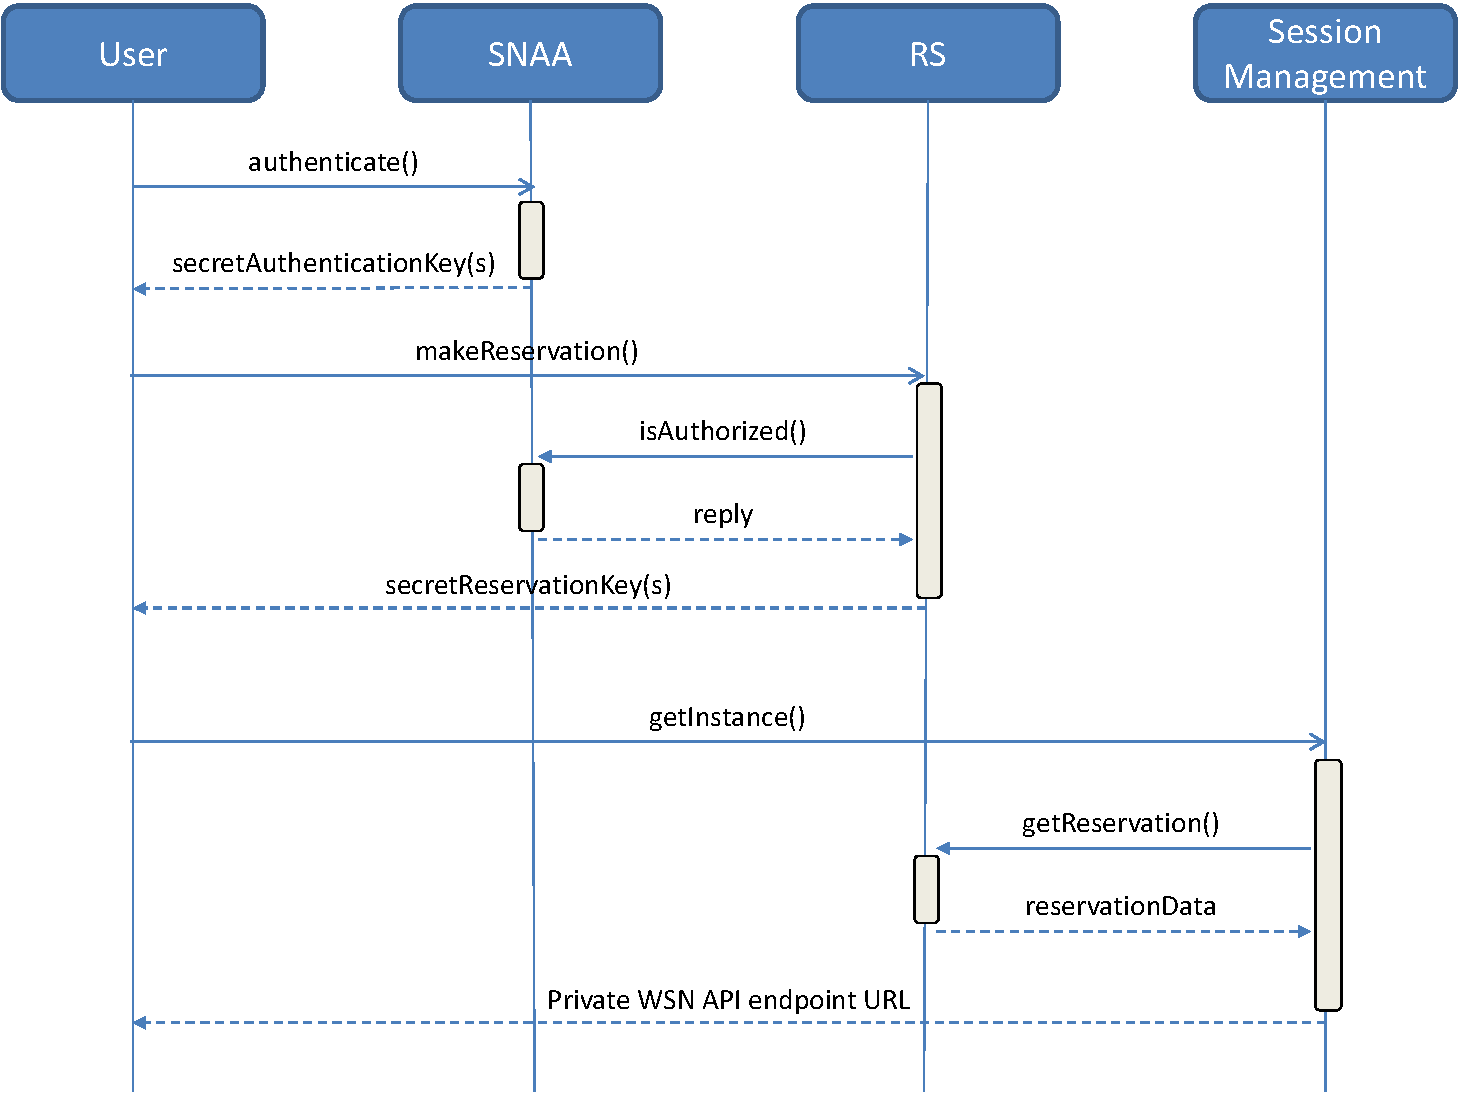
\includegraphics[width=.9\textwidth]{fig/api-sequence}
      \caption{Sequence of API calls}
      \label{fig:api-sequence}
      \end{center}
\end{figure*}

Since all APIs are federatable (i.e., the API for a federator is the same as for a single testbed), a user may potentially provide different authentication credentials for different (federated) testbeds. Hence, he does not provide a single \lstinline{<username,password>}-tuples, but a sequence of \lstinline{<username,password,urnprefix>}-tuples. The \lstinline{urnprefix} identifies the testbed (or again federation) to which the credentials belong. 
Hence, the resulting secret authentication key is not a simple string but also sequence of \lstinline{<urnprefix,key>}-tuples. Figure~\ref{fig:example-authenticate-request} and Figure~\ref{fig:example-authenticate-response} provide an example for this case. 

\begin{figure*}[htb]
      \begin{center}
      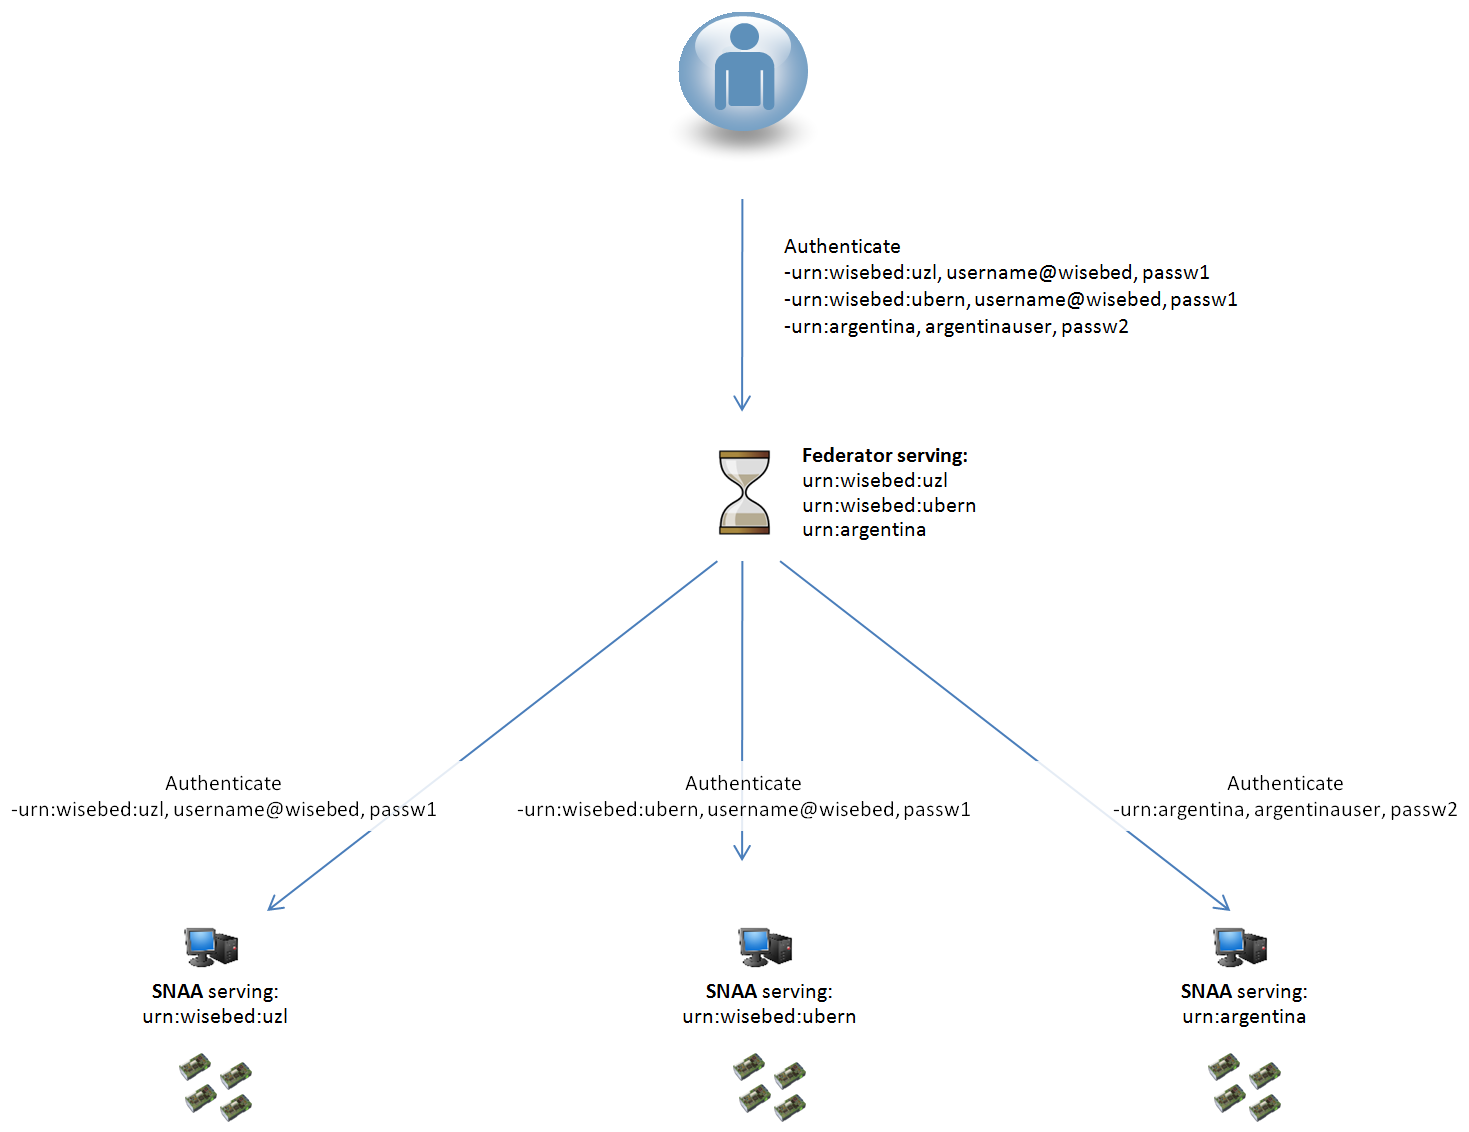
\includegraphics[width=.8\textwidth]{fig/example-authenticate-request}
      \caption{Request phase of the authenticate operation}
      \label{fig:example-authenticate-request}
      \end{center}
\end{figure*}

\begin{figure*}[htb]
      \begin{center}
      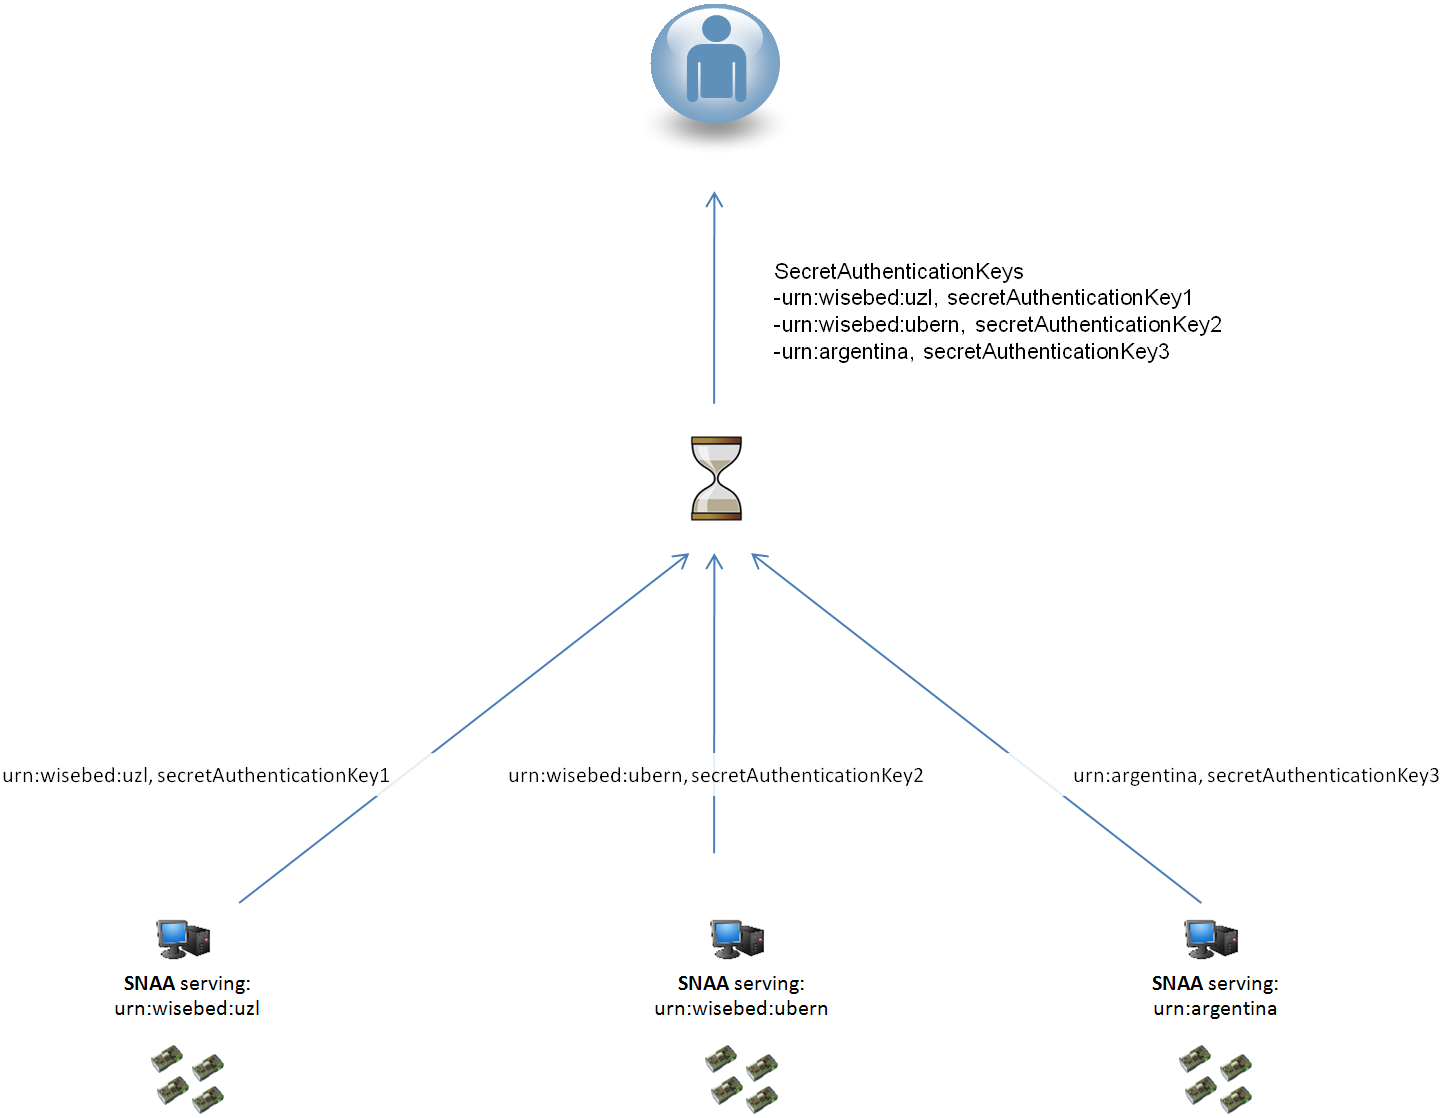
\includegraphics[width=.8\textwidth]{fig/example-authenticate-response}
      \caption{Response phase of the authenticate operation}
      \label{fig:example-authenticate-response}
      \end{center}
\end{figure*}

{\bf Important things to note:}

\begin{itemize}

	\item This requires that the \emph{user must trust the federator} and the \emph{federator must trust the individual backend implementations} since the user's password is passed on to these instances. This also requires that \emph{secure Web Service transport protocols should be used} (e.g., HTTPS or WS-Encryption) which is out of scope of this document.

	\item Within WISEBED, the password is only passed to a WISEBED-federator implementation which authenticates against a Shibboleth~\cite{shibboleth} federation and returns WISEBED-wide secret authentication keys and the local SNAA's only perform authorization.

	\item An implementation of the SNAA API may choose to serve only one URN prefix. If a request contains more than one of the aforementioned \lstinline{<username,password,urnprefix>}-tuples it must then throw an SNAAException fault (cf. Section~\ref{sec:faults}).

\end{itemize}

\FloatBarrier

%---------------------------------------------------------------------------
			\subsection{Authentication}
			\label{sec:authentication}
%---------------------------------------------------------------------------

\begin{apidoc}
	{List<SecretAuthenticationKey> authenticate(List<AuthenticationTriple> authenticationData) throws AuthenticationExceptionException, SNAAExceptionException;} %Signature
	{Returns a list of authentication keys for a set of credentials or signals a fault otherwise} % Semantics
	{
			\apiparameters{
				\apiparam{authenticationData}{List of $(urnprefix, username, password)$ tuples}
			}
	} % Parameters
	{A $(urnprefix, secretauthenticationkey)$ tuple for corresponding input tuple or a fault otherwise} % Returns
	{} % Rationale for addition/changes
	{1.0} % Since
\end{apidoc}

This function is about authentication of users. It accepts a sequence of $(urnprefix, username, password)$ tuples and returns a $(urnprefix, secretauthenticationkey)$ tuple for corresponding input tuple or a fault otherwise. Figure~\ref{fig:authenticate-request} visualizes the input and Figure~\ref{fig:authenticate-response} visualizes the structure of the response. This function completes without a fault only if authentication is successful for ALL of the supplied input tuples. Otherwise, it will signal an AuthenticationExceptionException. If some other fault occurs, it will signal a generic SNAAExceptionException fault (cf. Section~\ref{sec:faults}). Upon success, it must return a $(urnprefix, secretauthenticationkey)$ tuple for each $urnprefix$ supplied as input. 

An implementation of this API function may choose to only accept a single-entry list (e.g., because it only serves a single URN prefix) while another implementation (e.g., a federator) may accept crendentials for more than one URN prefix. 

	\myfig[.8\textwidth]{authenticate-request}{Authentication Request}
	\myfig[.8\textwidth]{authenticate-response}{Authentication Response}
	
%---------------------------------------------------------------------------
			\subsection{Authorization}
			\label{sec:authorization}
%---------------------------------------------------------------------------

\begin{apidoc}
	{public boolean isAuthorized(List<SecretAuthenticationKey> authenticationData, Action action) throws SNAAExceptionException;} %Signature
	{Asks for authorization for a given action.} % Semantics
	{
			\apiparameters{
				\apiparam{authenticationData}{A sequence of $(urnprefix, secretauthenticationkey)$ tuples. These were obtained from a call to authorize().}
				\apiparam{action}{The action for which authorization is requested.}
			}
	} % Parameters
	{true if authorization is granted, false otherwise} % Returns
	{} % Rationale for addition/changes
	{1.0} % Since
\end{apidoc}

This function is invoked by, e.g., the Reservation System, to ensure that an already authenticated used has the necessary rights to execute a certain action. The request and response messages of this function are visualized in Figure~\ref{fig:isauthorized-request} and \ref{fig:isauthorized-response}.

	\myfig[\textwidth]{isauthorized-request}{isAuthorized Request}
	\myfig[0.6\textwidth]{isauthorized-response}{isAuthorized Response}

%---------------------------------------------------------------------------
			\subsection{Fault Messages}
			\label{sec:faults}
%---------------------------------------------------------------------------
This section summarizes the possible faults signaled by the functions of this API. 
Figure~\ref{fig:authentication-fault} visualizes the structure of a fault signaled when authentication fails and  Figure~\ref{fig:snaa-fault} shows the structure of a generic, possibly internal, fault.

	\myfig[0.6\textwidth]{authentication-fault}{Authentication Fault}
	\myfig[0.6\textwidth]{snaa-fault}{SNAA Fault}

%--------------------------------------------------------------------------------------------------------
	\sectionfin
	\section{Appendix}
	\label{sec:appendix}		
%--------------------------------------------------------------------------------------------------------
    
%---------------------------------------------------------------------------
			\subsection{WSDL}
%---------------------------------------------------------------------------

    	\lstinputlisting[language=WSDL,tabsize=1,basicstyle=\scriptsize]{../wsdl/SNAA.wsdl}

%---------------------------------------------------------------------------
			\subsection{Data Types (XML Schema)}
%---------------------------------------------------------------------------

    	\lstinputlisting[language=XMLSchema,tabsize=1,basicstyle=\scriptsize]{../wsdl/SNAATypes.xsd}

%--------------------------------------------------------------------------------------------------------
%--  References
%--------------------------------------------------------------------------------------------------------
	\sectionfin
	\addcontentsline{toc}{section}{References}
	\bibliographystyle{abbrv}
	\bibliography{references}

	\label{lastpage}
\end{document}
